\section{Estado del arte}
\subsection{Búsquedas Scopus}
\begin{frame}
    \frametitle{Tendencia Scopus}
    \begin{columns}
      \column{0.5\textwidth}
      \begin{figure}
        \begin{center}
          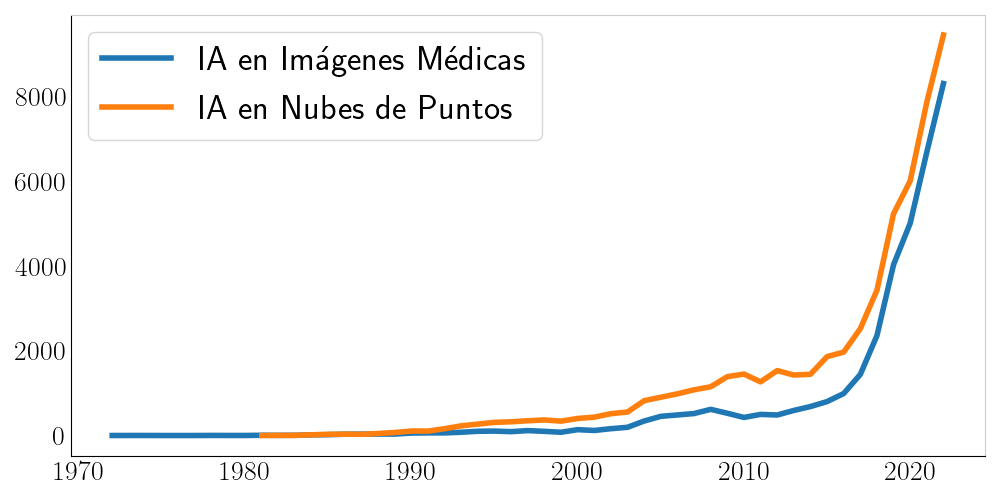
\includegraphics[width=\textwidth]{imagenes/chapter2/ScopusMLinMedicineAndPC}
        \end{center}
        \caption{Aprendizaje automático en medicina (azul) y nubes de puntos (naranja).
        \textbf{Ambos superan los 6000 documentos}.}
      \end{figure}
      
      \column{0.5\textwidth}
      \begin{figure}
        \begin{center}
          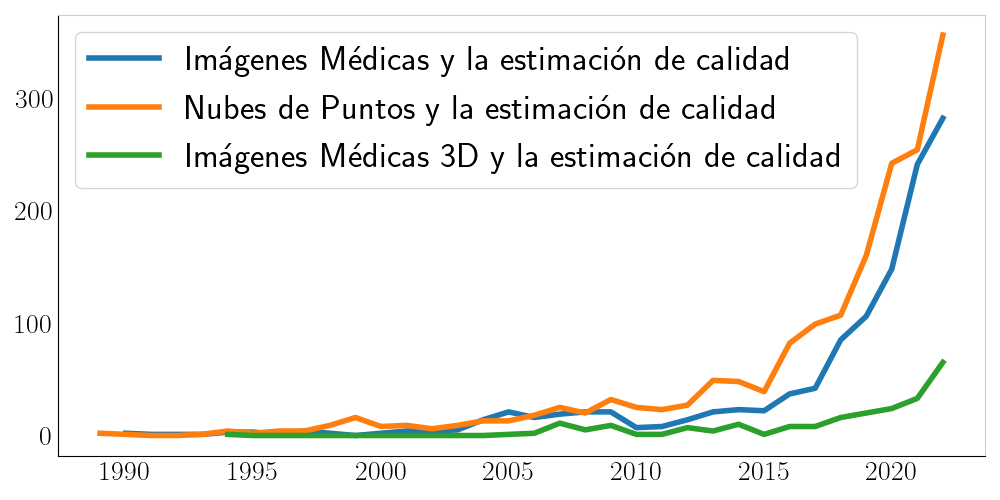
\includegraphics[width=\textwidth]{imagenes/chapter2/ScopusQualityAssessment}
        \end{center}
        \caption{Estimación de calidad en imágenes médicas (azul), nubes de puntos (naranja) 
          y en imágenes médicas 3D (verde). Esta última, tan solo llega a \alert{60 publicaciones}}
      \end{figure}
    \end{columns}
\end{frame}

\subsection{Estado del arte IQA}
\begin{frame}
  \frametitle{Estado del arte FR-IQA}
  \begin{columns}
    \column{0.5\textwidth}
    \begin{enumerate}
      \item Están basados en los avances del conocimiento sobre el sistema visual humano (HVS):
        \begin{enumerate}[<+->]
          \item Cuantificación de la señal. 
          \item La \textbf{sensibilidad al contraste}.
          \item Hipótesis de percepción a través de: brillo, contraste y \alert{estructuras}.
          \item La \textbf{saliencia visual}. 
          \item Empleo de \textbf{modelos DL}.
        \end{enumerate}
    \end{enumerate}

    \column{0.5\textwidth}
  \begin{table}[htp]
    \footnotesize
    \centering
    \begin{tabular}{|c|c|c|c|}
      \hline
      \rowcolor[HTML]{FFC702}
      \cellcolor[HTML]{FFC702} &  \multicolumn{3}{c|}{\cellcolor[HTML]{FFC702}\textbf{LIVE}}\\ \cline{2-4}
      \rowcolor[HTML]{FFC702}
      \multirow{-2}{*}{\textbf{Métrica}} & SRCC & PLCC & RMSE \\ 
      \hline
                    \alert<1-2>{PSNRHVS} & 0.919 & 0.903 & 12.540 \\
                     UQI & 0.894 & 0.899 & 11.982 \\
                     \alert<3>{SSIM} & 0.948 & 0.845 & 8.946 \\
                     \alert<4>{VSI} & 0.952 & 0.948 & 8.682 \\
                     DSS & 0.962 & 0.931 & 9.961 \\
                     \alert<5>{CD-MMF} & \textbf{0.981} & \textbf{0.980} & \textbf{5.413}\\ 
                     WaDIQaM & 0.970 & \textbf{0.980} & - \\
                    \hline 
    \end{tabular}
    \caption[Progreso de las métricas FR.]{
      Progreso de las métricas FR conforme avanza los conocimientos del HVS, ML y DL\footnotemark.
      }
      \label{tab:SOTAFRIQA}
  \end{table}
  \end{columns}
\footcitetext{SurveyOf2D3DMetrics}
\end{frame}

\begin{frame}
  \frametitle{Estado del arte NR-IQA}
  \begin{columns}
    \column{0.5\textwidth}
    \begin{enumerate}[<+->]
      \item Métricas basadas en \textbf{tipos específicos de distorsiones}.
      \item Métricas basadas en \alert{estadísticas de escenas naturales} (NSS).
      \item Métricas basadas en \textbf{aprendizaje automático}.
      \item Métricas basadas en \alert{aprendizaje profundo}.
    \end{enumerate}
    \column{0.5\textwidth}
    \begin{table}[htp]
        \footnotesize
        \centering
        \begin{tabular}{|c|c|c|c|}
        \hline 
        \rowcolor[HTML]{FFC702}
        \cellcolor[HTML]{FFC702} & \multicolumn{3}{c|}{\cellcolor[HTML]{FFC702}\textbf{LIVE}} \\ \cline{2-4}
        \rowcolor[HTML]{FFC702}
          \multirow{-2}{*}{\textbf{Métrica}} & SROCC & PLCC & RMSE \\
        \hline
                              \alert<2>{BRISQUE} & 0.940 & 0.942 & - \\
                               \alert<3>{LGP} & 0.957 & 0.954 & 7.901 \\
                               IQA-CNN & 0.956 & 0.953 & - \\
                               DIQaM-NR & \textbf{0.960} & \textbf{0.972} & - \\
                               \alert<4>{Hallucinated-IQA} & \textbf{0.982} & \textbf{0.982} & - \\
                              \hline
      \end{tabular}
      \caption[Tablas estado del arte NR-IQA.]{
        Progreso de las métricas NR al utilizar métodos cada vez más complejos\footnotemark.}
      \label{tab:SOTANRIQA}
    \end{table}
  \end{columns}
\footcitetext{SurveyOf2D3DMetrics}
\end{frame}

\subsection{Estado del arte PCQA}
\begin{frame}
  \frametitle{Estado del arte PCQA}
  \begin{columns}
    \column{0.5\textwidth}
    \begin{enumerate}[<+->]
      \item Extracción de características del vecindario del punto.
        \begin{enumerate}
          \item Características \textbf{geométricas}.
          \item Características \textbf{lumínicas}.
        \end{enumerate}
      \item Métodos para casos específicos. 
      \item Métodos genéricos por ML. 
      \item Métodos genéricos por DL.
        \begin{enumerate}
          \item \textbf{Proyecciones 2D.}
          \item \textbf{Interpretación 3D directa.}
          \item Mixto.
        \end{enumerate}
    \end{enumerate}

    \column{0.5\textwidth}
      \begin{table}[htp]
          \footnotesize
          \centering
          \begin{tabular}{|c|c|c|c|c|}
              \hline
              \rowcolor[HTML]{FFC702}
              \cellcolor[HTML]{FFC702} & \multicolumn{2}{c|}{\cellcolor[HTML]{FFC702}\textbf{STJU-PCQA}} & \multicolumn{2}{c|}{\cellcolor[HTML]{FFC702}\textbf{WPC}} \\ 
              \cline{2-5}
             \multirow{-2}{*}{\cellcolor[HTML]{FFC702}\textbf{MODELO}}  &\multicolumn{1}{c|}{\cellcolor[HTML]{FFC702} PLCC} & \multicolumn{1}{c|}{\cellcolor[HTML]{FFC702}SRCC} & \multicolumn{1}{c|}{\cellcolor[HTML]{FFC702}PLCC} & \multicolumn{1}{c|}{\cellcolor[HTML]{FFC702}SRCC} \\
              \hline
              IT-PCQA & 0.58 & 0.63 & 0.55  & 0.54\\
              \hline
              \alert<3->{NR3DQA} & 0.7382 & 0.7144 & 0.6514 & 0.6479\\
              \hline
              GPA-Net & 0.806 & 0.78 & - & - \\
              \hline
              ResSCNN & 0.86 & 0.81 & 0.72 & 0.75\\
              \hline
              \alert<4->{VQA-PC} & 0.8635 & 0.8509 & 0.7976 & 0.7968\\
              \hline
              MM-PCQA & \textbf{0.92} & \textbf{0.91} & \textbf{0.83} & \textbf{0.83}\\
              \hline
          \end{tabular}
          \caption[Estado del arte de modelos NR-PCQA]{
          Resumen del estado del arte de modelos NR-PCQA en dos datasets SJTU y WPC.
        }
      \end{table}
  \end{columns}
\end{frame}

\subsection{Estado del arte en imágenes médicas}
\begin{frame}
  \frametitle{Estado del arte en imágenes médicas}
  \begin{enumerate}
    \item \textbf{No existe} una imagen o representación \alert{``sin distorsión''} en la medicina.
    \item Los métodos \textbf{actuales} utilizan adaptaciones \textbf{IQA} para 
      exámenes médicos específicos como \textbf{MRI}.
    \item No se ha encontrado nada específico en la literatura sobre 
      métodos aplicados a reconstrucciones 3D.
  \end{enumerate}
\end{frame}
